\documentclass[10pt]{beamer}

\usepackage{settings}
\usepackage


\title{Causal Effect Variational Autoencoder}
\subtitle{Final Exam Project}
\date{June 17, 2025}
\author[longname]{Valeria De Stasio, Christian Faccio, Giovanni Lucarelli}
\titlegraphic{\hfill
\includegraphics[height=1.3cm]{images/logo100_orizzontale.pdf}}

% add graphics path
\graphicspath{{../assets},{./images}}

\begin{document}

\maketitle

% magari un frame iniziale in cui introduciamo il concetto di causalità?

%From "association" to "causation"
\begin{frame}{Objective: estimating causal effects}
  To estimate how a treatment $T$ affects an outcome $Y$, we would like to intervene on $T$ for \textit{random} subjects and observe the effect on $Y$. This corresponds to a Randomized Clinic Trial.
  \begin{figure}
    \centering
    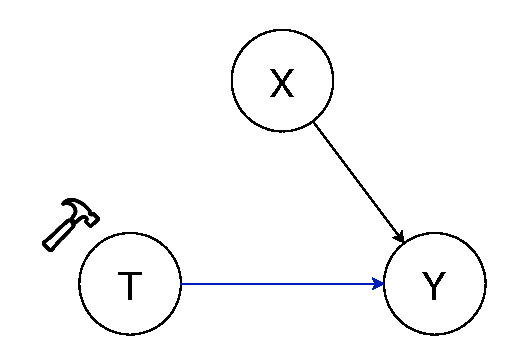
\includegraphics[width=0.5\textwidth]{images/intervention.drawio.pdf}
  \end{figure}
  \begin{equation*}
    P(Y|\text{do}(T=t))=P(Y|T=t)
  \end{equation*}
\end{frame}

% How to intervene on already observed data?
\begin{frame}{Confounder}
  In a observational study we do \textbf{not} have control over 
  $T$: there may be a confounder $X$ that influences both variables!
  
  If we observe all confounders $X$, then we can block the backdoor path and compute the causal effect of $T$ on $Y$.
  \begin{figure}
    \centering
    %RMK: all variables are observed...
    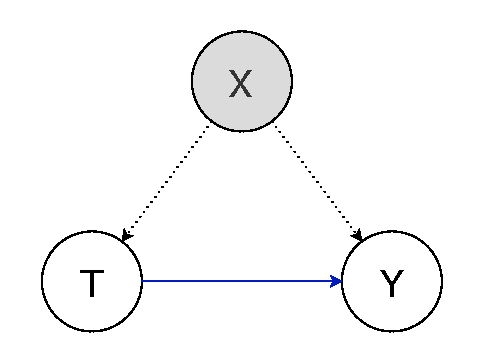
\includegraphics[width=0.5\textwidth]{images/backdoor.drawio.pdf}
  \end{figure}
  \begin{equation*}
    P(Y|\text{do}(T=t)) = \sum_{x} P(Y|T=t, X=x) P(X=x)
  \end{equation*}
\end{frame}

% magari possiamo fondere questa slide con la precedente!
%What if latent confounds are present?
\begin{frame}{Latent confounder}
  But what if there is a confounder $Z$ that is \textbf{not} observed? This is the most likely scenario in which $X$ is only a proxy for $Z$.

  This time the back-door criterion is not satisfied: we cannot compute the causal effect of $T$ on $Y$.

  \begin{figure}
    \centering
    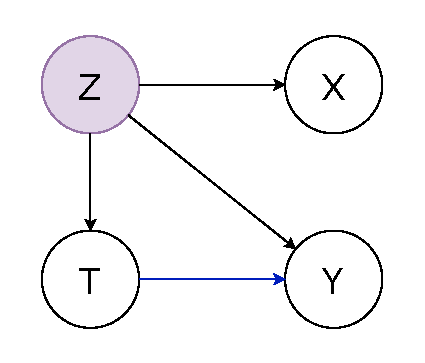
\includegraphics[width=0.5\textwidth]{images/latent.drawio.pdf}
  \end{figure}


\end{frame}

\begin{frame}{Synthetic dataset}
    \begin{minipage}
    [t]{0.5\textwidth}
      \begin{figure}
        \centering
        \includegraphics[width=0.8\textwidth]{../images/synthetic_data.pdf}
      \end{figure}
    \end{minipage}
    \begin{minipage}
    [t]{0.5\textwidth}
      \begin{itemize}
        \item $T$ is a binary treatment
        \item $Y$ is a continuous outcome
        \item $X$ is a proxy for the latent confounder $Z$
        \item $Z$ is a continuous latent variable
      \end{itemize}
    \end{minipage}
\end{frame}

\begin{frame}{Experiment: noise in the proxies}
    
\end{frame}

\begin{frame}{Experiment: latent distribution misspecified}
    
\end{frame}

\begin{frame}{Experiment: changing latent dimension}
    
\end{frame}

\begin{frame}{Experiment: increasing the treatment effect}
    
\end{frame}

\begin{frame}{Conclusions}
    
\end{frame}

{\setbeamercolor{palette primary}{fg=white, bg=bluscuro}
\begin{frame}[standout]
\thispagestyle{empty}
  {\LARGE Thank You!}
\end{frame}
}



\end{document}